%!TEX root = qualificacao.tex
\section[REPRESENTAÇÃO DE PROPRIEDADES ESTÁTICAS POR MEIO DE TEMPLATES]{REPRESENTAÇÃO DE PROPRIEDADES \\ ESTÁTICAS POR MEIO DE TEMPLATES}
\label{sec:propriedadesEstaticas}

Em ACs, propriedades estáticas são propriedades computadas com base nas tabelas de transição. Essas propriedades permitem prever determinados comportamentos de um ACs sem consultar sua evolução espaço temporal. 

Esta seção descreverá algumas propriedades estáticas e os algoritmos geradores de templates que as representam. Todos algoritmos explicados estão implementados na biblioteca \textit{CATemplates} \cite{CATemplates}.

\subsection{Conservabilidade de Estados e Conservabilidade de Paridade}
Conservabilidade de estados é uma propriedade estática que determina que a soma dos estados de um determinado autômato celular não deve se alterar durante a evolução espaço temporal, independente da configuração inicial passada.

De acordo com Boccara e Fukś (\citeyear{boccara2002}), um AC é conservativo quando cada uma de suas regras locais $f$ de vizinhança $(\alpha_0,\alpha_1, \dots, \alpha_{n-1})$ respeita as condições descritas na Equação \ref{eq:conservativeCA}.

\begin{equation}
\begin{split}
f(\alpha_0,\alpha_1, \dots,\alpha_{n-1}) = \alpha_0 + (\sum_{i=0}^{n-2}f(0_0,0_1, \dots,0_i,\alpha_1,\alpha_2, \dots,\alpha_{n-1}) \\- f(0_0,0_1, \dots,0_i,\alpha_0,\alpha_1, \dots,\alpha_{n-i-1}))
\label{eq:conservativeCA}
\end{split}
\end{equation}

Para exemplificar, considere a regra 204 do espaço elementar. Por meio da condição mostrada na Equação \ref{eq:conservativeCA}, será provado que essa regra é conservativa, já que satisfaz a condição. A Equação \ref{eq:ruleTable204} representa a tabela de transições da regra 204.

\begin{equation}
\begin{split}
(((1,1,1),1),((1,1,0),1),\\((1,0,1),0),((1,0,0),0),\\((0,1,1),1),((0,1,0),1),\\((0,0,1),0),((0,0,0),0))
\label{eq:ruleTable204}
\end{split}
\end{equation}

Como demonstra \citeonline{Verardo2014}, a aplicação das condições da Equação \ref{eq:conservativeCA} nas tabelas de transições de ACs do espaço elementar, sempre resultará no sistema descrito pela Equação \ref{eq:conservativeLinearSystem}.

\begin{equation}
\left\{\begin{matrix}
 f(0,0,0) = 0 + (f(0,0,0) - f(0,0,0)) + (f(0,0,0) - f(0,0,0))\\ 
 f(0,0,1) = 0 + (f(0,0,1) - f(0,0,0)) + (f(0,0,0) - f(0,0,0))\\ 
 f(0,1,0) = 0 + (f(0,1,0) - f(0,0,1)) + (f(0,0,1) - f(0,0,0))\\ 
 f(0,1,1) = 0 + (f(0,1,1) - f(0,0,1)) + (f(0,0,1) - f(0,0,0))\\ 
 f(1,0,0) = 1 + (f(0,0,0) - f(0,1,0)) + (f(0,0,0) - f(0,0,1))\\ 
 f(1,0,1) = 1 + (f(0,0,1) - f(0,1,0)) + (f(0,0,0) - f(0,0,1))\\ 
 f(1,1,0) = 1 + (f(0,1,0) - f(0,1,1)) + (f(0,0,1) - f(0,0,1))\\ 
 f(1,1,1) = 1 + (f(0,1,1) - f(0,1,1)) + (f(0,0,1) - f(0,0,1))
\end{matrix}\right.
\label{eq:conservativeLinearSystem}
\end{equation}

A Equação \ref{eq:conservativeLinearSystem} simplificada é representada pela Equação \ref{eq:conservativeLinearSystem2}.

\begin{equation}
\left\{\begin{matrix}
 f(0,0,0) & = & 0 		& &\\ 
 f(0,0,1) & = & f(0,0,1)& & \\ 
 f(0,1,0) & = & f(0,1,0)& & \\ 
 f(0,1,1) & = & f(0,1,1)& & \\ 
 f(1,0,0) & = & 1 - f(0,0,1) - f(0,1,0) \\ 
 f(1,0,1) & = & 1 - f(0,1,0) \\ 
 f(1,1,0) & = & 1 + (f(0,1,0) - f(0,1,1))\\ 
 f(1,1,1) & = & 1 & &
\end{matrix}\right.
\label{eq:conservativeLinearSystem2}
\end{equation}

Excluindo-se as condições tautológicas do sistema e atribuindo os valores das funções locais $f$ conforme a tabela de transições da regra 204, é obtido o sistema descrito pela Equação \ref{eq:conservativeAC204}. Esse sistema, ao não apresentar condições contraditórias ou falsas, prova que a regra 204 é conservativa.

\begin{equation}
\left\{\begin{matrix}
 0 & = & 0 \\ 
 0 & = & 1 - 0 - 1 \\ 
 0 & = & 1 - 1 \\ 
 1 & = & 1 + (1 - 1)\\ 
 1 & = & 1 
\end{matrix}\right.
\label{eq:conservativeAC204}
\end{equation}

O algoritmo que gera templates que representam regras conservativas, criado por De Oliveira e Verardo (\citeyear{deOliveira2014}), primeiramente recebe as variáveis $k$ e $r$ definindo assim a família das regras que serão geradas. Em seguida, cria todas as vizinhanças do espaço com exceção das vizinhanças que geram tautologias. E após esses passos, aplica as condições de Boccara e Fukś (\citeyear{boccara2002}). Para se excluir as vizinhanças que geram tautologias, basta excluir as vizinhanças que começam com 0 mas não sejam compostas apenas por 0 \cite{Schranko2010}.

Para exemplificar o funcionamento do algoritmo, considere um espaço com $k=2$ e $r=1$. Primeiramente o algoritmo obterá o conjunto das vizinhanças que não geram regras tautológicas, portanto será obtido o conjunto $\{(1,1,1),(1,1,0),(1,0,1),(1,0,0),(0,0,0)\}$. Então é criado o sistema de equações \ref{eq:conservativeLinearSystem3}, baseado nas condições de Boccara e Fukś (\citeyear{boccara2002}).

\begin{equation}
\left\{\begin{matrix}
 x_0 & = & 0\\ 
 x_4 & = & 1 +2x_0 -x_1 -x_2\\ 
 x_5 & = & 1 +x_0 -x_2\\
 x_6 & = & 1 +x_2 -x_3\\ 
 x_7 & = & 1
\end{matrix}\right.
\label{eq:conservativeLinearSystem3}
\end{equation}

Por fim o algoritmo utiliza a função Solve do \textit{Wofram Mathematica} para simplificar o sistema e utiliza o conjunto solução retornado pela função Solve como regras de substituições. Essas regras de substituições são aplicadas no template base, gerando assim o template das regras conservativas. O template gerado pode ser observado na Equação \ref{eq:conservativeTemplate}, e sua expansão gera as cinco regras conservativas do espaço elementar, após eliminadas as regras inválidas.

\begin{equation}
(1,x_2-x_3+1,1-x_2,-x_1-x_2+1,x_3,x_2,x_1,0)
\label{eq:conservativeTemplate}
\end{equation}

O processo de gerar regras conservativas de paridade é bem parecido. Porém as condições estabelecidas por Boccara e Fukś (\citeyear{boccara2002}) são ligeiramente modificadas em relação a Equação \ref{eq:conservativeCA}, de forma que cada uma das funções locais deve respeitar agora as condições da Equação \ref{eq:parityConservativeCA}.

\begin{equation}
\begin{split}
f(\alpha_0,\alpha_1, \dots,\alpha_{n-1}) \equiv \alpha_0 + (\sum_{i=0}^{n-2}f(0_0,0_1, \dots,0_i,\alpha_1,\alpha_2, \dots,\alpha_{n-1}) \\- f(0_0,0_1, \dots,0_i,\alpha_0,\alpha_1, \dots,\alpha_{n-i-1})) \; (mod 2)  
\label{eq:parityConservativeCA}
\end{split}
\end{equation}

A biblioteca \textit{CATemplates} já tem implementado o algoritmo gerador de templates de regras conservativas de paridade, e conforme será mostrado posteriormente, esse algoritmo pode ser de suma importância na busca de uma solução para o problema de paridade.





\subsection{Confinamento}
Os autômatos celulares confinados, ou \textit{captive} em Inglês, são uma classe de AC que se baseiam em uma caracterização de suas funções locais que não adotem estados definidos em qualquer estrutura externa à vizinhança \cite{theyssier2004captive}. 

\citeonline{theyssier2004captive} formalmente define que dado a função local $f$ de um AC para a vizinhança $(\alpha_0, \dots, \alpha_{2r})$, sendo o $r$ o raio, um AC é considerado confinado se respeitar a condição descrita na Equação \ref{eq:captiveAC}.

\begin{equation}
f((\alpha_0, \dots, \alpha_{2r})) = \beta, \beta \in \{\alpha_0, \dots, \alpha_{2r}\}
\label{eq:captiveAC}
\end{equation}

Essa propriedade pode ser facilmente representada através de templates. Para isto, basta restringir as variáveis a um conjunto de valores presentes na vizinhança correspondente. A biblioteca \textit{open source CATemplates} já apresenta um algoritmo que gera as regras confinadas. Esse algoritmo recebe como parâmetro os argumentos $k$ e $r$. Após isso, gera as vizinhanças do espaço e verifica em cada uma das vizinhanças os estados que elas têm. Caso a vizinhança tenha todos os estados do intervalo $[0, k-1]$ essa posição terá uma variável livre no template. Caso a vizinhança tenha apenas um estado a posição correspondente no template assume um valor fixo. Por fim, caso a vizinhança apresente mais de um estado, mas não todos, a posição correspondente do template apresentará uma variável restritas mediante expressões $x_i \in C$.

É trivial perceber que qualquer AC binário que tenha as funções locais $f((0_0, 0_1,\dots, 0_{2r})) = 0$ e $f((1_0, 1_,1\dots, 1_{2r})) = 1$ é caracterizado como um AC confinado. A Equação \ref{eq:captiveTemplateACE} representa o template de todas as regras confinadas do espaço elementar e as equações \ref{eq:captiveTemplateR05} representam a família de $k=2$ e $r=0,5$.
\begin{equation}
(1,x_6,x_5,x_4,x_3,x_2,x_1,0)
\label{eq:captiveTemplateACE}
\end{equation}

\begin{equation}
(1,x_2,x_1,0)
\label{eq:captiveTemplateR05}
\end{equation}

Por fim, a Equação \ref{eq:captiveTemplateK3} representa a família dos autômatos celulares confinados de $r=1$ e três estados.

\begin{equation}
\begin{split}
(2, x_{25} \in \{1,2\}, x_{24} \in \{0,2\}, x_{23} \in \{1,2\}, x_{22} \in \{1,2\}, x_{21}, x_{20} \in \{0,2\}, x_{19}, x_{18} \in \{0,2\}, \\
x_{17} \in \{1,2\}, x_{16} \in \{1,2\}, x_{15}, x_{14} \in \{1,2\},1, x_{12} \in \{0,1\}, x_{11}, x_{10} \in \{0,1\}, x_9 \in \{0,1\}, \\
x_8 \in \{0,2\}, x_7, x_6 \in \{0,2\}, x_5, x_4 \in \{0,1\}, x_3 \in \{0,1\}, x_2 \in \{0,2\}, x_1 \in \{0,1\}, 0)
\label{eq:captiveTemplateK3}
\end{split}
\end{equation}

\subsection{Simetria Interna}

\subsection{Invariância a Troca de Cor}

\subsection{Totalidade e Semi-totalidade}
Os ACs totalísticos são autômatos celulares cujo valor de uma célula depende apenas da soma dos valores dos seus vizinhos no passo de tempo anterior \cite{wolfram1983statistical}.

De forma análoga é possivel dizer que as transições dependem da médias das células que compõem  a vizinhança ao invés da soma. A Figura \ref{fig:totalistcRule} ilustra o a tabela de transição do AC totálistico 777 com $k = 3$ e $r = 1$. 
	\begin{figure}[h!]
	  \centering
	  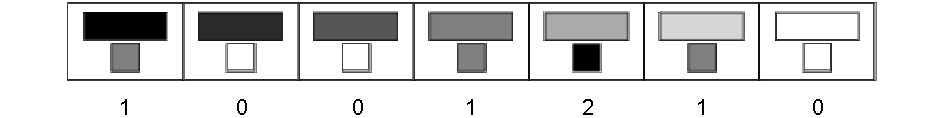
\includegraphics[width=1\textwidth]{fig_totalistcRule777.pdf}
	  \caption{Tabela de transição do AC totálistico 777. As transições dependem da média dos estados das células da vizinhança. Cada média possível é representada por tons de cinza entre o branco (estado 0) e o preto (estado 2).}
	  \label{fig:totalistcRule}
	\end{figure}

Já os ACs semi-totalísticos (\textit{outer-totalistic CA}) são generalizações de ACs totalísticos \cite{weisstein2015outerTotalistic}. Um AC pode ser considerado semi-totalístico caso suas transições sejam definidas pela soma (ou média) das células da vizinhança entretanto sem levar em consideração a célula central.

%talvez trocar citação de Gardner.
O Jogo da Vida \cite{GardnerM1970} é o exemplo mais conhecido de autômatos celulares semi-totalisticos, além de apresentar propriedades bem interessantes, como a computabilidade universal.

Os ACs semi-totalísticos podem ser interpredos como ACs clássicos que apresentam a propriedade de \textit{semi-totalidade}. A propriedade de semi-totalidade determina que as as trasições que apresentem a mesma soma dos estados vizinhos externos e que tenham a mesma célula central devem apresentar o mesmo resultado. Da mesma forma os AC totalísticos também tem sua propriedade correspondente nos ACs clássicos: a \textit{totalidade}. A totalídade determina que todas as trasições que apresente a mesmo soma dos estados das vizinhanças devem levar a um mesmo resultado.

A partir das definições de como devem ser as transições de estados dos ACs totalísticos e dos ACs semi-totalísticos foi possível representa-los através de templates. A biblioteca \textit{CATemplates} já apresenta os algoritmos que as geram essa propriedades e seu funcionamento é bem simples. 

O algoritmo que gera regras totalísticas recebe como argumento os valores de $r$ e $k$, definindo assim uma família de ACs. Em seguida enumera as vizinhanças do espaço e calcula a soma dos estados de cada uma delas. O resultados da soma é o que define quais transições devem ser iguais para que o template represente apenas regras totalísticas.

Para determinar qual será a váriavel associada, dada uma vizinhança qualquer, o agoritmo verifica se a vizinhança foi a única até então que obteve um determinado valor de soma. Em caso positivo o algoritmo criará e associará uma variável $x_i$ para esta transição, sendo $i$ o valor decimal da vizinhança. Caso contrário, a transição será associada uma váriavel $x_i$ em que $i$ é o valor decimal da primeira e menor vizinhança encontrada com o mesmo valor de soma das vizinhanças.

 